\documentclass[fontsize=12pt]{article}
%\documentclass[journal]{IEEEtran}
%\documentclass[conference]{IEEEtran}
\usepackage[a4paper, total={6.5in, 9in}]{geometry}
\usepackage{datetime}
\usepackage{graphicx}
\usepackage[rightcaption]{sidecap}
\usepackage{hyperref}
\usepackage{amsmath}
\usepackage{amssymb}
\usepackage[resetlabels,labeled]{multibib}


\begin{document}

% title and author part starts

\title{Department of Computer Science \&  Engineering \\ Chittagong University Of Engineering \& Technology \\ Chittagong-4349\\ 
	\noindent\rule{13cm}{0.4pt}\\
	 Course Code: CSE - 458\\Course Title: Graphics Design (Sessional)\\
	\noindent\rule{13cm}{0.4pt}\\
}

% enter author names

\author {
	Fariha Iffath, ID: 1304120\\	
}
\date{March 22, 2019}

\maketitle
\newpage

\pagenumbering{arabic}

\section{Objective} % (fold)

to develop a suitable graphics package to simulate the Windmill and to implement the skills learned in Interactive Computer Graphics  using OpenGL.

\section{Introduction}

Computer graphics is concerned with all aspects of producing pictures or images using a computer. The field began humbly almost 50 years ago, with the display of a few lines on a cathode-ray tube (CRT). Now, we can create images by computer that are indistinguishable from photographs of real objects. We routinely train pilots with simulated airplanes, generating graphical displays of a virtual environment in real time\cite{R:1}.\\
Feature-length movies made entirely by computer have been successful, both critically and financially. Massive multiplayer games can involve tens of thousands of concurrent participants. Visualization is any technique for creating images, diagrams or animations to communicate a message\cite{R:2}.

\subsection{Simuation \& Animation}

Classical graphics techniques arose as a medium to convey information among people.	We have computer plotting packages that provide a variety of plotting techniques and color tools that can handle multiple large data sets. The field of information visualization is becoming increasingly more important as we have to deal with understanding complex phenomena from problems in bioinformatics to detecting security threats.\\

Once graphics systems evolved to be capable of generating sophisticated images in real time, engineers and researchers began to use them as simulators. One of the most important uses has been in the training of pilots. Graphical flight simulators have proved to increase safety and to reduce training expenses. The use of special VLSI chips has led to a generation of arcade games s as sophisticated as flight simulators.\\

\subsection{User Interfaces}

Interaction with computers has become dominated by a visual paradigm that includes windows, icons, menus, and    plotting device, such as mouse. User interfaces demonstrate the variety of the tools available in high level modeling packages and the interactive devices the user can employ in modeling geometric object.

\subsection{Image Types}
    \textbf{2D Computer Graphics} are the computer-based generation of digital images mostly from two-dimensional models, such as 2D geometric models, text, and digital images, and by techniques specific to them.2D computer graphics are mainly used in applications that were originally developed upon traditional printing and drawing technologies, such as typography, cartography, technical drawing, advertising. Two-dimensional models are preferred, because they give more direct control of the image than 3D computer graphics, whose approach is more akin to photography than to typography.\\

    \textbf{3D Computer Graphics} in contrast to 2D computer graphics are graphics that use a three-dimensional representation of geometric data that is stored in the computer for the purposes of performing calculations and rendering 2D images.\\

\subsection{OpenGL}

As a software interface for graphics hardware, OpenGL's main purpose is to render two- and three-dimensional objects into a frame buffer. These objects are described as sequences of vertices (which define geometric objects) or pixels (which define images). OpenGL\cite{R:3} performs several processing steps on this data to convert it to pixels to form the final desired image in the frame buffer.\\

\subsection{$<$Glut.h$>$}

GLUT is the OpenGL Utility Toolkit, a window system independent toolkit for writing OpenGL programs. It implements a simple windowing application programming interface (API) for OpenGL. GLUT makes it considerably easier to learn about and explore OpenGL programming. GLUT provides a portable API so you can write a single OpenGL program that works on both Win32 PCs and X11 workstations\cite{R:4}.\\

GLUT is designed for constructing small to medium sized OpenGL programs. While GLUT is well-suited to learning OpenGL and developing simple OpenGL applications, GLUT is not a full-featured toolkit so large applications requiring sophisticated user interfaces are better off using native window system toolkits like Motif. GLUT is simple, easy, and small.

\section{Overview of The Project}
\begin{enumerate}
\item we designed the simulation of windmill using OpenGL. We used transformation functions like translate and rotate functions to design blades of the windmill. We used many OpenGL inbuilt function to design the structure of windmill.
\item This project consist of many user defined function such as increasing windmill fan speed, decreasing windmill fan speed, side views, front and back views, custom angle of rotation of entire windmill structure.
\item It provides several options which can be interacted through menus. The user can also interact with program through mouse, keyboard functions. The options provided by the menu are views like side view, back view, front view, custom view. Using mouse, if we click left side, it rotates to left and on successive clicking speed increases, if we click right button, speed decreases and on successive clicking, it turns rotating towards right and vice versa.
\item We can rotate the entire windmill with respect to its axis using the arrow keys of keyboard. It can be rotated through $360^{0}$.
\end{enumerate}

\section{Requirements Specification}

\subsection{Functional Requirements}
It describes what the system should do.
\begin{enumerate}
\item Simulation of Windmill should be implemented by using keyboard and mouse.
\item Sequence of menus should be displayed on pressing middle mouse button as shown:
	\begin{enumerate}
		\item Side View 1
		\item Side View 2
		\item Back View
		\item Front View
		\item Custom View
	\end{enumerate}
\item On pressing left mouse button, the windmill wheel starts rotating and on further clicks the speed of rotation increases.
\item On pressing right mouse button, the rotating speed of the windmill wheel slows down and finally comes to halt. 
\item Simulation of Windmill shall also be done using the keys-\\
 Right Arrow and Left Arrow keys are used to rotate the whole Windmill Structure.
\end{enumerate}

\subsection{Software}
\begin{enumerate}
\item Operating System		: Windows 10
\item Programming Language	: C, C++
\item Toolkit				: Glut Toolkit
\end{enumerate}

\section{Design}

The flow of control in the flow chart below is respected to the Texture Package. For any of the program flow chart is compulsory to understand the program. We consider the flow chart for the texture project in which the flow starts from start and proceeds to the main function after which it comes to the initialization of call back functions and further it proceeds to mouse and keyboard functions after all the function, the flow comes to quit which is the end of the flow chart. 

\begin{figure}[h]
	\centering
  	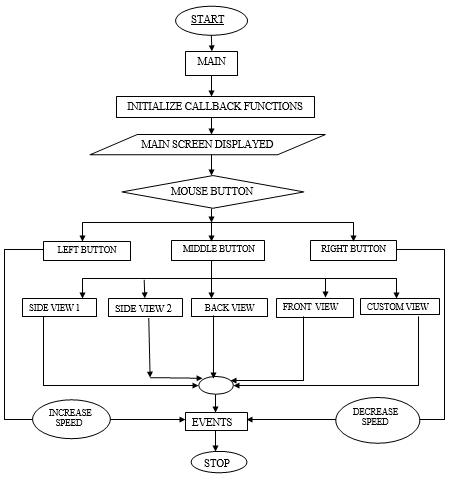
\includegraphics{Flow_Chart.PNG}
  	\caption{Flow Chart for Simulation of Windmill}
  	\label{fig:FlowChart}
\end{figure}

\section{Implementation}

\begin{verbatim}

#include <GL/glut.h>
#include<stdio.h>
#include<conio.h>
#define M_SIDE1 20
#define M_SIDE2 21
#define M_BACK  22
#define M_FRONT 23
#define M_CUSTOM 24
#define SIZE 500

float x_angle = 0.0;
float y_angle = 0.0;
float z_angle = 0.0;
float camera_angle=0.0;
float c=1.0;

GLfloat pos[] = { 0.0, 0.0, -10.0, 1.0 };
GLfloat white[] = { 2.5, 2.5, 6.0, 6.0 };
GLfloat red[] = { 0.7, .4, 0.0, 1.0 };
GLfloat deep_blue[] = { 0.3, 0.3, 0.9, 1.0 };
GLfloat shiny[] = { 50.0 };
GLfloat dull[] = { 0.0 };
GLUquadricObj *Cylinder;
enum { X, Y, Z } axis = X;

void change_view (int sel) {

switch (sel)
{

    case M_CUSTOM:{	printf("ENTER VIEWANGLE:");
                                	scanf("%f",&camera_angle); }
                                 	break;
    case M_SIDE1: {camera_angle=90;}
                           		break;
    case M_SIDE2: camera_angle=-90;
                           		break;
    case M_BACK: camera_angle=180;
                           		break;
    case M_FRONT:camera_angle=0;
    default: break; }
}

void initialize_menu (void)
{

    glutCreateMenu(change_view );
    glutAddMenuEntry("SIDE VIEW 1", 20);
    glutAddMenuEntry("SIDE VIEW 2", 21);
    glutAddMenuEntry("BACK VIEW", 22);
    glutAddMenuEntry("FRONT VIEW", 23);
    glutAddMenuEntry("CUSTOM VIEW", 24);
    glutAttachMenu(GLUT_MIDDLE_BUTTON);
}

void mouse_button (int button, int state, int x, int y)
{

    if (button == GLUT_LEFT_BUTTON )
    {
                      axis=Z; c=c+0.4;
                      printf("WIND SPEED INCREASE\t SPEED=%fKm/Hr\n\n",c*1.5);
                      glutPostRedisplay();
    }

    else if (button == GLUT_RIGHT_BUTTON )
    {
                      axis = Z; c=c-0.4;
                      printf("WIND SPEED DECREASE\t SPEED=%fKm/Hr\n\n",c*1.5);
                      glutPostRedisplay();
    }
}

void spin(void)
{
         switch (axis)
                  {
                      case X: x_angle += 1.0;
                                   break;
                      case Y: y_angle += 1.0;
                                   break;
                      case Z: z_angle += c ;
                                   break;
                      default: break;
                  }

         glutPostRedisplay();
}

void display (void)
{

    Cylinder = gluNewQuadric();
    gluQuadricDrawStyle( Cylinder, GLU_FILL);
    gluQuadricNormals( Cylinder, GLU_SMOOTH);
    gluQuadricOrientation( Cylinder, GLU_OUTSIDE );
    glClear(GL_COLOR_BUFFER_BIT | GL_DEPTH_BUFFER_BIT);
    glMatrixMode(GL_MODELVIEW);
    glLoadIdentity();
    glEnable(GL_TEXTURE_2D);
      
    //Bottom
   glTexParameteri(GL_TEXTURE_2D,GL_TEXTURE_MIN_FILTER,
                              GL_NEAREST);
   glTexParameteri(GL_TEXTURE_2D, GL_TEXTURE_MAG_FILTER,
                               GL_NEAREST);
   glMaterialfv(GL_FRONT, GL_AMBIENT, white);

   glBegin(GL_QUADS);
        glNormal3f(0.0, 1.0f, 0.0f);
        glTexCoord2f(0.0f, 0.0f);
        glVertex3f(-25.0,-25.0,-44);
        glTexCoord2f(0.0f, 1.0f);
        glVertex3f(-25.0,25.0,-44);
        glTexCoord2f(1.0f, 1.0f);
        glVertex3f(25.0,25.0,-44);
        glTexCoord2f(1.0f, 0.0f);
        glVertex3f(25.0,-25.0,-44);

   glEnd();
   glDisable(GL_TEXTURE_2D);
   glRotatef(camera_angle,0.0,1.0,0.0);
   gluCylinder(Cylinder,.4,.4,4,16,20);
   glMaterialfv(GL_FRONT_AND_BACK, GL_AMBIENT_AND_DIFFUSE, red);
   glMaterialfv(GL_FRONT_AND_BACK, GL_SPECULAR, red);
   glMaterialfv(GL_FRONT_AND_BACK, GL_SHININESS, shiny);
   glPushMatrix();
   glutSolidTorus (1.4, 1.4,  6,  6);
   glutSolidCube(2.5);
   glPushMatrix();
   glTranslatef(0.0,-2.0,0.0);
   glMaterialfv(GL_FRONT_AND_BACK, GL_DIFFUSE, red); 

    //material property for the base of the windmill
   glMaterialfv(GL_FRONT_AND_BACK, GL_SPECULAR, red);
   glPushMatrix();
   glRotatef(90.0,1.0,0.0,0.0);
   glTranslatef(0.0,0.0,-2.0);
   gluCylinder(Cylinder,1.0,1.5,27,50,50);
   glPopMatrix();
   glPopMatrix();
   glRotatef(z_angle, 0.0, 0.0, 1.0);
   glMaterialfv(GL_FRONT_AND_BACK, GL_AMBIENT_AND_DIFFUSE, red);
   glMaterialfv(GL_FRONT_AND_BACK, GL_SPECULAR, white);
   glPushMatrix();
   glTranslatef(0.0,0.0,1.5);
   glutSolidCone(1.5,2.5,50,50);
   glPopMatrix();
   glPushMatrix();		//blade 1
   glTranslatef(0.0,0.0,2.2);
   glRotatef(90.0,1.0,0.0,0.0);
   glPushMatrix();
   glRotatef(120,0.0,1.0,0.0);
   glutSolidCone(0.9, 16.0, 15, 15);
   glPopMatrix();
   glPopMatrix();
   glPushMatrix();		//blade 2
   glTranslatef(0.0,0.0,2.2);
   glRotatef(90.0,1.0,0.0,0.0);
   glPushMatrix();
   glRotatef(-120,0.0,1.0,0.0);
   glutSolidCone(0.9, 16.0, 15, 15);
   glPopMatrix();
   glPopMatrix();
   glPushMatrix();		 //blade 3 
   glTranslatef(0.0,0.0,2.2);
   glRotatef(90.0,1.0,0.0,0.0);
   glutSolidCone(0.9, 16.0, 15, 15);
   glPopMatrix();
   glLightfv(GL_LIGHT1, GL_POSITION, pos);
   glutSwapBuffers();
}

void init (void)
{
   glMatrixMode(GL_PROJECTION);
   glLoadIdentity();
   glOrtho(-25.0, 25.0, -25.0, 25.0, -250.0, 250.0);
   glEnable(GL_LIGHTING);
   glEnable(GL_LIGHT0);
   glEnable(GL_LIGHT1);
   glEnable(GL_NORMALIZE);
}

void special (int key, int x, int y) 
{
    switch (key)
   {
    case GLUT_KEY_LEFT: {axis = X; camera_angle--;
                   printf("\n\nVIEW ANGLE=%f", camera_angle);};
                   glutPostRedisplay();
                   break;
    case GLUT_KEY_RIGHT: {axis = Y; camera_angle++;
                   printf("\n\nVIEW ANGLE=%f", camera_angle);};
                   glutPostRedisplay();
                   break;
    case GLUT_KEY_UP: c=c+0.4; 
                   glutPostRedisplay();
                   break;	
    case GLUT_KEY_END:  exit(0); 	
    case GLUT_KEY_DOWN:{c=c-0.4;};
                   glutPostRedisplay();
                   break;
    default: break;
    }
}

void reshape (int width, int height)
{

    GLfloat w, h;
    glViewport(0, 0, width, height);
    glMatrixMode(GL_PROJECTION);
    glLoadIdentity();
    if (width > height)
    {
        w = (25.0 * width) / height;
        h = 25.0;
    }

    else
    {
        w = 25.0;
        h = (25.0 * height) / width;
    }

    glOrtho(-w, w, -h, h, -250.0, 250.0);
    glutPostRedisplay();
 }

void main (int argc, char *argv[ ])
{
    glutInit(&argc, argv);
    glutInitDisplayMode(GLUT_RGBA | GLUT_DOUBLE);
    glutInitWindowSize(SIZE, SIZE);
    glutInitWindowPosition(100, 50);
    glutCreateWindow("SIMULATION OF WINDMILL");
    glutIdleFunc(spin);
    glutDisplayFunc(display);
    glutSpecialFunc(special);
    glutMouseFunc(mouse_button);
    initialize_menu();
    glutReshapeFunc(reshape);

    init();

    glEnable(GL_DEPTH_TEST);
    glutMainLoop();
}
\end{verbatim}

\section{OpenGL Functions}
The project is implemented by using the below OpenGL functions:

\subsection{Window Manageent Function}
Six routines perform tasks necessary to initialize a window.

\begin{itemize}
\item \textbf{glutInit(int *argc, char **argv)} 
- Initializes GLUT. The arguments from main are passed in by the application.
\end{itemize}
\begin{itemize}
\item \textbf{glutInitDisplayMode(unsigned int mode)}
- Requests a display with the properties in mode. The value of mode is determined by the logical OR.
\end{itemize}
\begin{itemize}
\item \textbf{glutInitWindowPosition(int x, int y)}
- Specifies the screen location for the upper-left corner of your window.
\end{itemize}
\begin{itemize}
\item \textbf{glutInitWindowSize(int width, int size)}
- Specifies the size, in pixels, of your window.
\end{itemize}
\begin{itemize}
\item \textbf{int glutCreateWindow(char *string)}
- Creates a window on display. The string title can be used to label the window.
\end{itemize}
\begin{itemize}
\item \textbf{void glutMainLoop()}
- Cause the program to enter an event processing loop.
\end{itemize}

\subsection{Transformation Function}
\begin{itemize}
\item \textbf{void glRotatef( GLfloat angle, GLfloat x, GLfloat y, GLfloat z)}
- The glRotated and glRotatef functions multiply the current matrix by a rotation matrix.
\end{itemize}
\begin{itemize}
\item \textbf{void glTranslate(TYPEx, TYPEy, TYPEz)}
- The glTranslated and glTranslatef functions multiply the current matrix by a translation matrix.
\end{itemize}

\subsection{Call Back Function}
\begin{itemize}
\item \textbf{glutDisplayFunc(void (* func)(void))}
- Whenever GLUT determines the contents of the window need to be redisplayed, the callback function registered by glutDisplayFunc() is executed.
\end{itemize}
\begin{itemize}
\item \textbf{glutReshapeFunc}
- glutReshapeFunc sets the reshape callback for the current window.
\end{itemize}
\begin{itemize}
\item \textbf{void glutIdleFunc(void (*func)(void))}
- glutIdleFunc sets the global idle callback. This function is invoked when there are no other events. Its default is the NULL function pointer. A typical use of idle function is to continue to generate graphical primitives through a display function while nothing is happening.
\end{itemize}

\subsection{Interactive Function}
\begin{itemize}
\item \textbf{void glutKeyboardFunc(void (*func)(unsigned char key, int x, int y))}
- Registers the keyboard callback function 'func'. The callback function returns the ASCII code of the key pressed and the position of the mouse.
\end{itemize}
\begin{itemize}
\item \textbf{void glutMouseFunc(void (*func)(int button, int state, int x, int y))}
- Registers the mouse callback function 'func'. The callback function returns the button (GLUT \_LEFT \_BUTTON, GLUT \_RIGHT  \_BUTTON, GLUT \_MIDDLE \_BUTTON), the state of the button after the event (GLUT\_UP, GLUT\_DOWN) and the position of the mouse with respect to the top left corner of the window.
\end{itemize}
\begin{itemize}
\item \textbf{int glutCreateMenu(void (*func)(int value))}
- Returns an identifier for a top-level menu and registers the callback function f that returns an integer value corresponding to the menu entry selected. glutCreateMenu creates a new pop-up menu and returns a unique small integer identifier.
\end{itemize}
\begin{itemize}
\item \textbf{void glutAddMenuEntry(char *name, int value)}
- This function adds an entry with the string name displayed to the current menu. Value is returned to the menu callback when the entry is selected.
\end{itemize}
\begin{itemize}
\item \textbf{void glutAttachMenu(int button)}
- glutAttachMenu attaches a mouse button for the current window to the identifier of the current menu.
\end{itemize}
\begin{itemize}
\item \textbf{void glPushMatrix() \& void glPopMatrix}
- Push to and pops from the matrix stack corresponding to the current matrix mode.
\end{itemize}
\begin{itemize}
\item \textbf{void glOrtho(GLdouble left, GLdouble right, GLdouble top, GLdouble bottom, GLdouble near, GLdouble far)}
- Defines an Orthographic viewing volume with all parameters measured from the center of the projection plane.
\end{itemize}
\newpage
\section{Output}

\begin{figure}[h]
	\centering
  	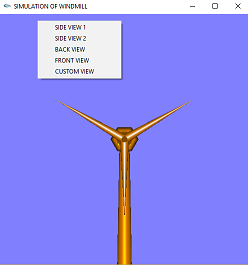
\includegraphics{F1.PNG}
  	\caption{Displaying the Menus with Front View}
  	\label{fig:Menus}
\end{figure}
The above diagram shows the snapshot having the windmill. The objects are of windmill shape and are placed towards the right of the display window and the display window is of size (600, 600). The diagram shows the snapshot having  menus which consists of front view, back view, side view 1, side view 2 and custom view.\\

\begin{figure}[h]
	\centering
  	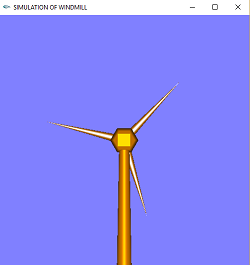
\includegraphics{F2.PNG}
  	\caption{Back View}
  	\label{fig:Back}
\end{figure}
The above diagram shows the snapshot about the option of Back View, in which the Back View of the Windmill structure is displayed.\\
\newpage

\begin{figure}[h]
	\centering
  	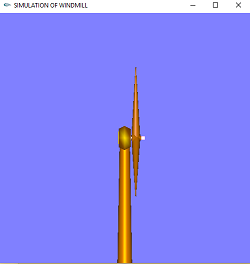
\includegraphics{F3.PNG}
  	\caption{Side View 1}
  	\label{fig:Side1}
\end{figure}
The above diagram shows the snapshot about the option of Side View, in which the Right view of the Windmill structure is displayed.\\

\begin{figure}[h]
	\centering
  	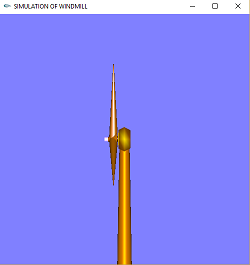
\includegraphics{F4.PNG}
  	\caption{Side VIew 2}
  	\label{fig:Side2}
\end{figure}
The above diagram shows the snapshot about the option of Side View , in which the Left view of the Windmill structure is displayed.\\
\newpage

\begin{figure}[h]
	\centering
  	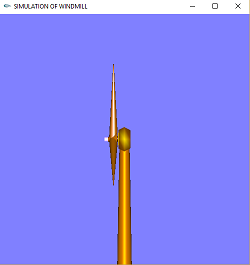
\includegraphics{F4.PNG}
  	\caption{Custom View with Angle $60^{0}$}
  	\label{fig:Custom}
\end{figure}

The above diagram shows the snapshot about free movement of the Windmill structure using the keys. The Right Arrow key is used to rotate the angle of the windmill structure clockwise, whereas the Left Arrow Key is used to rotate the angle of windmill structure anti-clockwise.\\

\begin{figure}[h]
	\centering
  	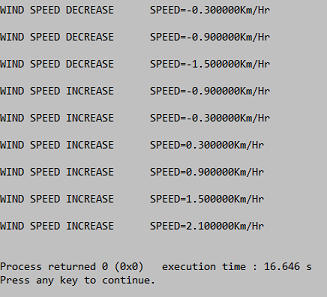
\includegraphics{F6.PNG}
  	\caption{Speed Tracking using Mouse Clicks}
  	\label{fig:Custom}
\end{figure}

The above diagram shows the snapshot about the simulation of the windmill. When the wheel of the windmill is made to rotate using the Left and Right Button of the mouse. When the Left Button of the mouse is clicked, it starts rotating and on further clicks the speed of the rotation increases. When the Right Button of the mouse is clicked, the rotation speed decreases and finally comes to halt.


\section{Conclusion}
\begin{enumerate}
\item Simulation of Windmill is designed and implemented using a graphics software system called OpenGL which has become a widely accepted standard for developing graphic application. Using OpenGL functions, user can create geometrical objects and can use translation, rotation, scaling with respect to the co-ordinate system.
\item The development of the Simulation of Windmill project has given us a good exposure to OpenGL by which we have learnt some of the techniques.
\item Simulation of Windmill consists of many user defined functions such as increasing windmill fan speed, decreasing windmill fan speed, side views, front and back views, custom angle of rotation of entire windmill structure. All these function makes this project an example of animation in OpenGL.
\end{enumerate}

\bibliography{citations}

\bibliographystyle{ieeetr}

\end{document}
